The implemented solution is organised into \textbf{three layers} (Figure~\ref{fig:exec_full_architecture}). The Streaming Core Layer extracts historical race data, creates replayable event records, streams them through Kafka, and processes them with Flink. The Evaluation and Modelling Layer converts persisted stream artifacts into Parquet datasets, builds the target contracts, trains and evaluates the Batch and MOA learners, and aligns the systems for comparison. The Delivery Layer produces reports, figures, audit tables, and validation outputs.

\begin{figure}[t]
    \centering
    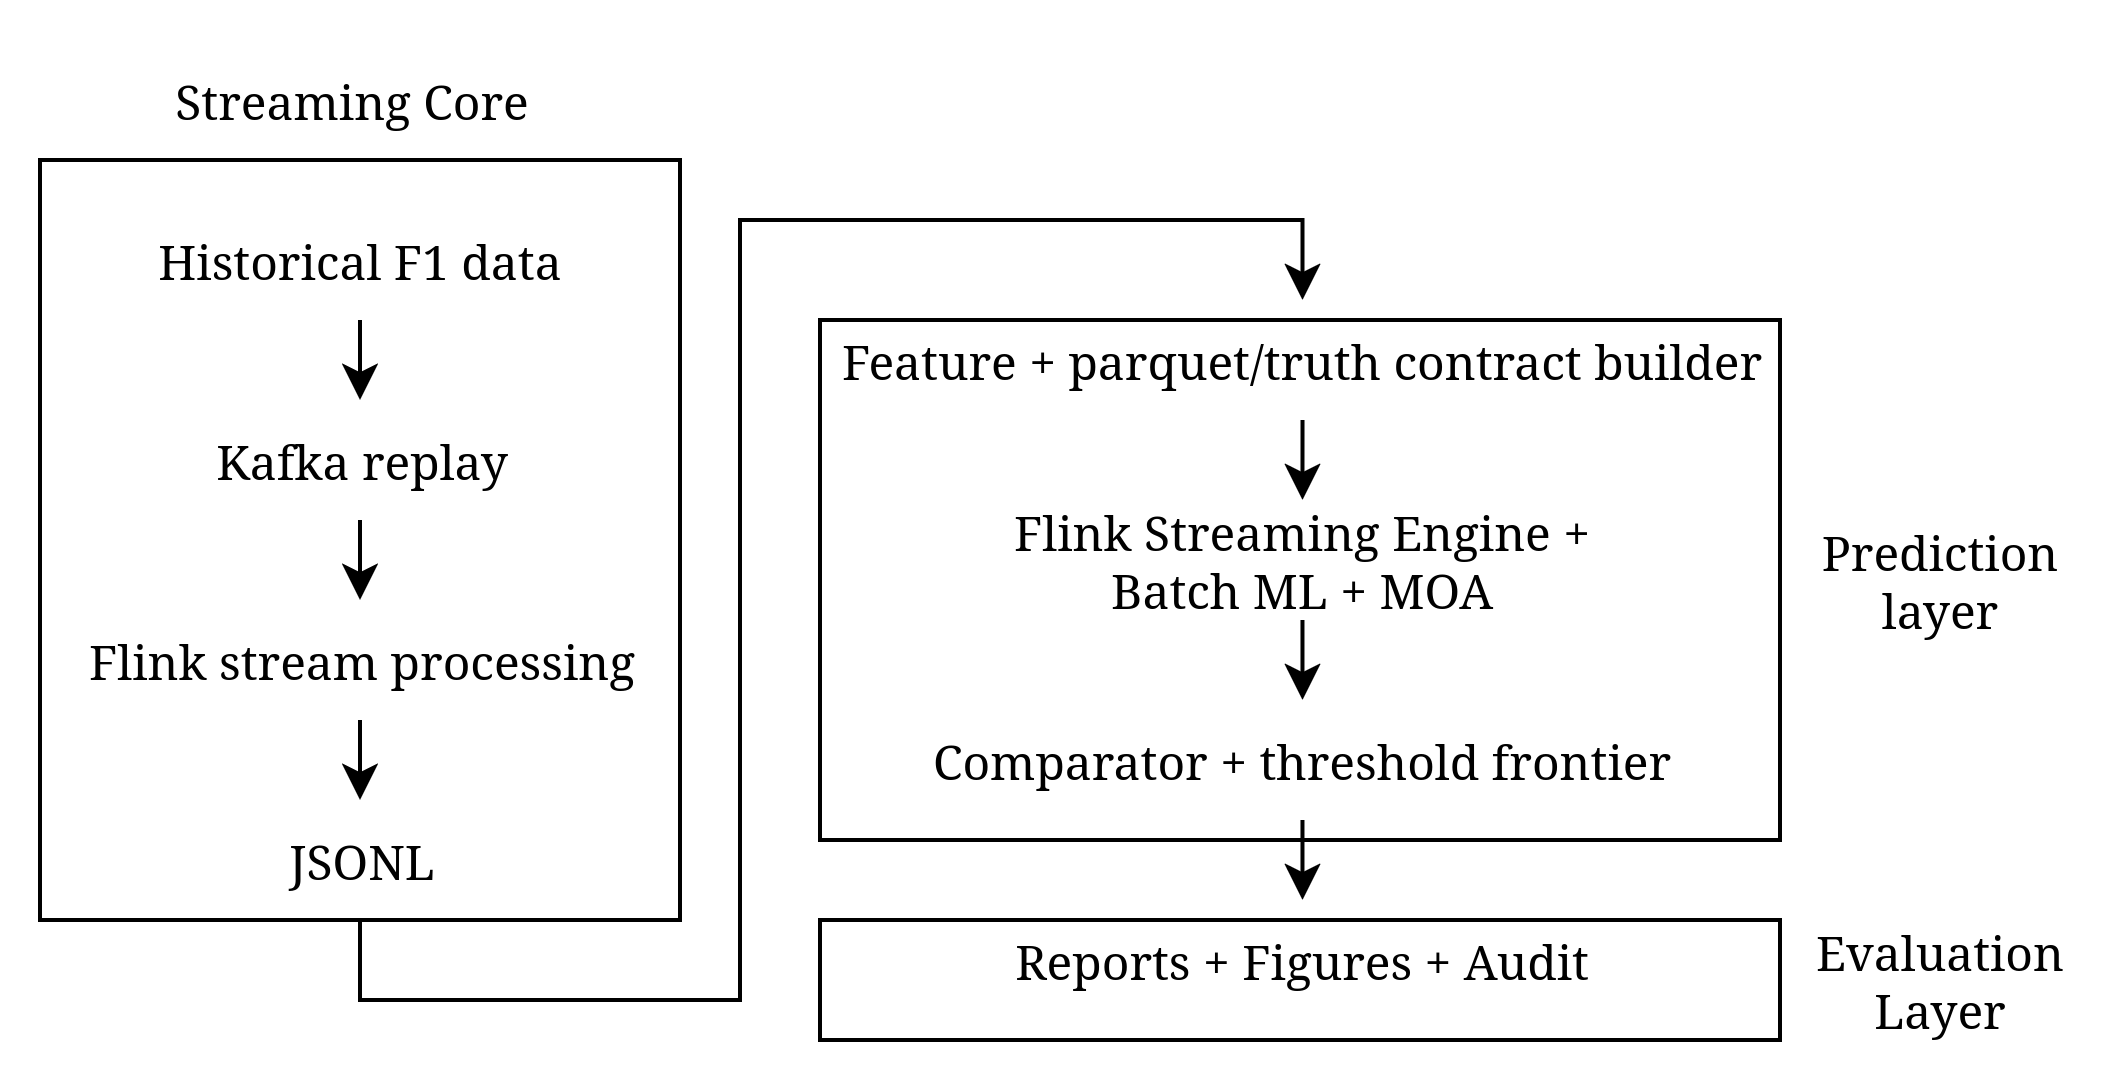
\includegraphics[width=\columnwidth]{Images/ch4/full_architecture.png}
    \caption{Pipeline architecture from historical race extraction to streaming, learning, and comparison.}
    \label{fig:exec_full_architecture}
\end{figure}

The ingestion stage starts from a race preparation script. FastF1 sessions are loaded and converted into a race snapshot containing lap events, telemetry-related observations, track status changes, weather, stint information, pit stop evidence, and race metadata. Lap events are enriched with team and stint data, total laps, pit-loss estimates, and available gap information. Events are then sorted by absolute timestamp and replayed through Kafka topics, so the historical race becomes an ordered log.

The Flink job consumes the replay topics and builds the \textbf{live race context} with \textbf{event-time processing}. Track status is broadcast to the operators that need it, while driver streams are keyed by race and driver. This allows stateful operators to maintain stint-specific and driver-specific information. Windowed computations group cars by race and lap to identify rivals ahead and behind, compute relevant gaps, and emit machine-learning feature rows as side outputs.

The stateful strategy logic produces several interpretable artifacts:
\begin{itemize}
    \item a tyre drop detector, which keeps the best lap in the current stint and counts consecutive slow laps;
    \item a drop-zone evaluator, which estimates where the driver would rejoin after a pit stop;
    \item a pit stop evaluator, which labels real pit outcomes from post-pit evidence;
    \item a pit suggestion stream, which scores whether the current context supports MONITOR, GOOD\_PIT, or PIT\_NOW.
\end{itemize}

The \textbf{Flink Strategy Engine} is the deterministic baseline. Its score combines pace loss, track status, traffic, strategic pressure, actionability, timing, end-of-race effects, competitive advantage, and uncertainty penalties. The final profile used in the evaluation is a guarded variant: rival pressure can increase urgency, but only when timing, gap, and traffic conditions support the call.

The \textbf{Batch path} uses the same artifacts to build supervised learning matrices for XGBoost. The matrix builder removes leakage-prone columns such as target labels, matched pit evidence, truth-lens flags, eligibility indicators, and metadata. Two feature profiles are compared: No-Year, which removes \texttt{source\_year} after it was identified as a shortcut risk, and Percent, which emphasises race-relative quantities such as race progress and lap-time ratios.

The \textbf{online path} exports the shared matrix logic to ARFF and evaluates MOA learners prequentially. Each instance is first scored, then used for training. The Java vote logger records labels, hard predictions, class votes, and a positive score derived from the vote distribution. These outputs are reconstructed with metadata so that MOA can be compared with Batch and Flink under the same threshold and event-matching logic.

A substantial part of the design is devoted to \textbf{fairness corrections}. The comparator aligns systems on the same race-driver universe, applies the same horizon, distinguishes raw and clean truth lenses, and evaluates both row-level and event-level behaviour. This prevents an implementation detail, such as missing outputs for one driver or a different denominator, from becoming a misleading performance gain.
